\section{Power Optimized Software Envelope}

\begin{figure}
\centering
\usepgfplotslibrary{fillbetween}

%Fix Area legend to not draw surrounding box
%Taken from http://tex.stackexchange.com/questions/99861/remove-border-around-area-legend-rectangle
\pgfplotsset{
    /pgfplots/area legend/.style={%
        /pgfplots/legend image code/.code={%
            \fill[##1] (0cm,-0.1cm) rectangle (0.6cm,0.1cm);
        }%
    },
}

\begin{tikzpicture}
  \begin{axis}[ticks = none, 
    axis on top,
    axis x line=bottom,
    axis y line=left,
  	xlabel={Runtime \emph{(s)}},
    ylabel={Energy \emph{(J)}},    
    xmin=0, xmax=50,
    ymin=0, ymax=3300,
    width=\linewidth,
    legend style={legend pos=north west}
    ]

    %% Model Parameters %%
    \pgfmathsetmacro{\baselinepower}{30} % NOP code
    \pgfmathsetmacro{\rooflinepower}{60}
    \pgfmathsetmacro{\codepower}{(\baselinepower*3 + \rooflinepower*4) / 7}
    \pgfmathsetmacro{\codetime}{30}
    % Sadly, pgfplots sucks too much to calculate cube roots
    \pgfmathsetmacro{\anodex}{26.20741}
    \pgfmathsetmacro{\anodey}{\anodex * \baselinepower}
    \pgfmathsetmacro{\cnodex}{34.34143}
    \pgfmathsetmacro{\cnodey}{\cnodex * \baselinepower}
    \pgfmathsetmacro{\tnodex}{27.25681}
 
    %% Intermezzo Values %%
    \pgfmathsetmacro{\codeenergy}{\codepower * \codetime}
    \pgfmathsetmacro{\baselineenergy}{\baselinepower * \codetime}
    \pgfmathsetmacro{\rooflineenergy}{\rooflinepower * \codetime}
    \pgfmathsetmacro{\lowdisplayline}{(2 * \baselinepower + \codepower) / 3}
    \pgfmathsetmacro{\highdisplayline}{(1 * \rooflinepower + 1 * \codepower) / 2}
    \pgfmathsetmacro{\rooflinetime}{\codeenergy/\rooflinepower}
    \pgfmathsetmacro{\baselinetime}{\codeenergy/\baselinepower}

    % arguments: code power, code time, x - todo, apparently not supposed to do pgfmathparse
    \pgfmathdeclarefunction{metricbound}{3}{%
      \pgfmathparse{((#1 * #2^3) / #3^2)}%
    }
    \pgfmathdeclarefunction{definitionbound}{3}{%
      \pgfmathparse{((#1 / #2^3) * #3^4)}%
    }
     \pgfmathdeclarefunction{optimizationlimits}{3}{%
      \pgfmathparse{(min(metricbound(#1, #2, #3), definitionbound(#1, #2, #3)))}
    }

    % BETA ROOFLINE BOUND
    \addplot[color=red, domain=\pgfkeysvalueof{/pgfplots/xmin}:\pgfkeysvalueof{/pgfplots/xmax}] {\rooflinepower * x};
    \addlegendentry{$P_{max}$ Energy Bound}

    %const power diagonal
    \addplot[color=darkgray, densely dashed, forget plot, %forget plot prevents legend entry
            domain=\pgfkeysvalueof{/pgfplots/xmin}:\pgfkeysvalueof{/pgfplots/xmax}] {\codepower * x}; 

    % ALPHA BASELINE BOUND 
    \addplot[color=green, domain=\pgfkeysvalueof{/pgfplots/xmin}:\pgfkeysvalueof{/pgfplots/xmax}] {\baselinepower * x};
    \addlegendentry{$P_{min}$ Energy Bound} 

    %Runtime Optimization
    \addplot[area legend, fill=blue, fill opacity=0.3, draw=none] coordinates { 
      (\codetime,\rooflineenergy)
      (\codetime,\baselineenergy)
    (0,0)};
    \addlegendentry{Runtime Optimization}

    %Power Optimization
    \addplot[area legend, fill=red, fill opacity=0.2, draw=none] coordinates {
                           (\codetime,\codeenergy)
                           (\pgfkeysvalueof{/pgfplots/xmax},\pgfkeysvalueof{/pgfplots/xmax}*\codepower)
                           (\pgfkeysvalueof{/pgfplots/xmax}, \pgfkeysvalueof{/pgfplots/xmax}*\baselinepower)
                           (0,0)
                         } ;
    \addlegendentry{Power Optimization}
  
    %Energy Optimization
    \addplot[area legend, style={pattern=north west lines, pattern color=gray,
                                 draw=none}] coordinates { 
      (\rooflinetime, \codeenergy)
      (\baselinetime, \codeenergy)
      (0, 0) };
    \addlegendentry{Energy Optimization}



    % Constant Time, Energy Dashes
    %vertical
    \draw[densely dotted] ({axis cs:\codetime,\baselineenergy}) -- ({axis cs:\codetime,\rooflineenergy});
    %horizontal
    \draw[densely dotted] ({axis cs:\rooflinetime,\codeenergy}) -- ({axis cs:\baselinetime,\codeenergy});
   

    \node[circle,fill,inner sep=2pt] at (axis cs:\codetime,\codeenergy) {};
    \node[below right] at (axis cs:\codetime,\codeenergy) {$\theta$};


 \end{axis}
\end{tikzpicture}

\caption{Feasible Performance Envelope}
\label{fig:motivation}
\end{figure}

The POSE heuristic is based on the notion of a feasible performance envelope like the one shown in \autoref{fig:motivation}.
This construct represents the set of all $(Runtime, Energy)$ costs it is possible for an arbitrary code to exhibit when running on a target platform. 

To build the feasible performance envelope we first plot a point corresponding to the measured energy and runtime costs of executing an unoptimized code $\theta$. 
We then plot lines of gradient $P_{max}$ and $P_{min}$ which represent the maximum and minimum bounds on system power consumption during normal operation.
By definition, all possible code executions on the target platform must correspond to a point within this envelope.




To constrain our search further we now consider the metric we wish to reduce. We know that for two logically equivalent codes $\theta$ and $\lambda$, the transformation $\theta \to \lambda$ is a valid optimization with respect to a cost metric $M$ if and only if $M(\lambda) < M(\theta)$. If we plot the curve linking all points having $M(\lambda) = M(\theta)$, then by definition any optimized versions of $\theta$ can only exist below this optimization bound. The exact equation of the curve depends on the chosen $E^mD^n$ metric as follows:

\begin{align}
E^mD^n(\theta) &= E^mD^n(\lambda) \nonumber \\
\implies {E_\lambda}^m &= \frac{{E_\theta}^m{D_\theta}^n}{{D_\lambda}^n} \nonumber \\
\implies E_\lambda &= (\frac{{E_\theta}^m{D_\theta}^n}{{D_\lambda}^n})^\frac{1}{m}
\end{align}

Our final bound considers what it means to optimize code for reduced power draw. We must avoid being too lenient; a large reduction in runtime associated with a negligible reduction in power draw should still be regarded as a classical optimization. On the other hand, our definition should include optimizations which deliver significant reductions in power draw with minuscule reductions in runtime. 

The definition we have settled on is that an optimization $\theta \to \lambda$ is a power optimization with respect to metric $M$ if the change in power draw it delivers is responsible for the majority of the reduction in $M$. Conversely, if the primary benefit of an optimization comes from improved runtime then it is to be considered a runtime optimization. We plot a curve linking those points which have the same ratio of contributions from both power and runtime factors to $M$ as our original code. All valid power optimizations must lie below this so-called contribution bound. Again the equation for this bound depends on the metric chosen and is derived as follows:

\begin{align}
\frac{{P_{\theta}}^m}{{D_{\theta}}^{m+n}} &= \frac{{P_{\lambda}}^m}{{D_{\lambda}}^{m+n}} \nonumber \\
\implies {P_{\lambda}}^m &= \frac{{P_{\theta}}^m}{{D_{\theta}}^{m+n}} \times {D_\lambda}^{m+n} \nonumber \\ 
\implies {E_{\lambda}}^m &= \frac{{P_{\theta}}^m}{{D_{\theta}}^{m+n}} \times {D_\lambda}^{m+n+1} \nonumber \\ 
\implies E_{\lambda} &= (\frac{{P_{\theta}}^m}{{D_{\theta}}^{m+n}} \times {D_\lambda}^{m+n+1})^{\frac{1}{m}} 
\end{align}

It may appear somewhat academic to base a bound on the definition of power optimization. That said, this is an important consideration in practice. Intuitively it makes sense to use the most appropriate tools while searching for optimizations. If code is sub-optimal and the penalty is felt more in one domain than the other then the tools and techniques developed for that domain are better suited to finding the optimization.

\begin{figure}
\centering
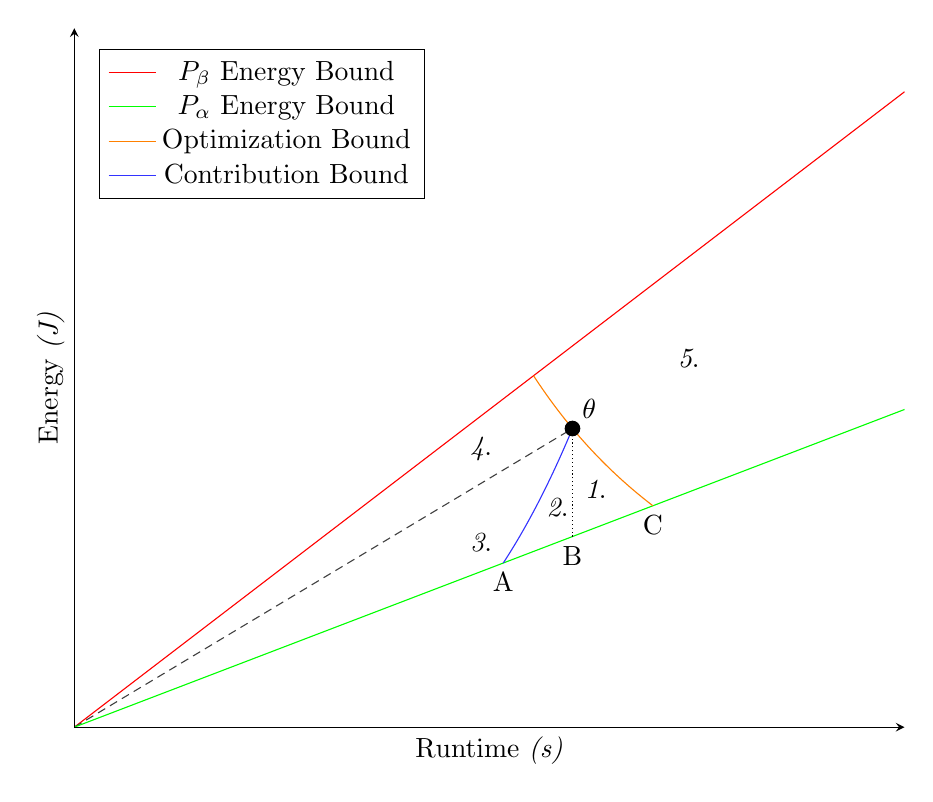
\begin{tikzpicture}
  \begin{axis}[ticks = none, 
    axis on top,
    axis x line=bottom,
    axis y line=left,
  	xlabel={Runtime \emph{(s)}},
    ylabel={Energy \emph{(J)}},    
    xmin=0, xmax=50,
    ymin=0, ymax=3300,
    width=\linewidth,
    legend style={legend pos=north west}
    ]

    %% Model Parameters %%
    \pgfmathsetmacro{\baselinepower}{30} % NOP code
    \pgfmathsetmacro{\rooflinepower}{60}
    \pgfmathsetmacro{\codepower}{47} 
    \pgfmathsetmacro{\codetime}{30}
    % Sadly, pgfplots sucks too much to calculate cube roots
    % These values are calculated with a ruby script in tools
    \pgfmathsetmacro{\anodex}{25.83028}
    \pgfmathsetmacro{\cnodex}{34.84283}
    \pgfmathsetmacro{\tnodex}{27.65477}

    \pgfmathsetmacro{\cnodey}{\cnodex * \baselinepower}
    \pgfmathsetmacro{\anodey}{\anodex * \baselinepower}
 
    %% Intermezzo Values %%
    \pgfmathsetmacro{\codeenergy}{\codepower * \codetime}
    \pgfmathsetmacro{\baselineenergy}{\baselinepower * \codetime}
    \pgfmathsetmacro{\rooflineenergy}{\rooflinepower * \codetime}
    \pgfmathsetmacro{\lowdisplayline}{(2 * \baselinepower + \codepower) / 3}
    \pgfmathsetmacro{\highdisplayline}{(1 * \rooflinepower + 1 * \codepower) / 2}

    % arguments: code power, code time, x - todo, apparently not supposed to do pgfmathparse
    \pgfmathdeclarefunction{metricbound}{3}{%
      \pgfmathparse{((#1 * #2^3) / #3^2)}%
    }
    \pgfmathdeclarefunction{definitionbound}{3}{%
      \pgfmathparse{((#1 / #2^3) * #3^4)}%
    }

    % BETA ROOFLINE BOUND
    \addplot[color=red, domain=\pgfkeysvalueof{/pgfplots/xmin}:\pgfkeysvalueof{/pgfplots/xmax}] {\rooflinepower * x};
    \addlegendentry{$P_{\beta}$ Energy Bound}

    %const power diagonal
    \addplot[color=darkgray, densely dashed, forget plot, %forget plot prevents legend entry
            domain=\pgfkeysvalueof{/pgfplots/xmin}:\codetime] {\codepower * x}; 

    % ALPHA BASELINE BOUND 
    \addplot[color=green, domain=\pgfkeysvalueof{/pgfplots/xmin}:\pgfkeysvalueof{/pgfplots/xmax}] {\baselinepower * x};
    \addlegendentry{$P_{\alpha}$ Energy Bound} 

    \addplot[color=orange, domain=\tnodex:\cnodex] { metricbound(\codepower, \codetime, x)};
    \addlegendentry{Optimization Bound}

    \addplot[color=blue!80, domain=\anodex:\codetime] { definitionbound(\codepower, \codetime, x)};
    \addlegendentry{Contribution Bound}

    % Constant Time, Energy Dashes
    %vertical
    \draw[densely dotted] ({axis cs:\codetime,\baselineenergy}) -- ({axis cs:\codetime,\codeenergy});

    \node[circle,fill,inner sep=2pt] at (axis cs:\codetime,\codeenergy) {};
    \node[above right] at (axis cs:\codetime,\codeenergy) {$\theta$};
    \pgfmathsetmacro{\oneycoord}{\lowdisplayline * 31.4}
    \node at (axis cs:31.4,\oneycoord) {\textit1.};
    \pgfmathsetmacro{\twoycoord}{\lowdisplayline * 29.1}
    \node at (axis cs:29.1,\twoycoord) {\textit2.};
    \pgfmathsetmacro{\threeycoord}{\lowdisplayline * 24.5}
    \node at (axis cs:24.5,\threeycoord) {\textit3.};
    \pgfmathsetmacro{\fourycoord}{\highdisplayline * 24.5}
    \node at (axis cs:24.5,\fourycoord) {\textit4.};
    \pgfmathsetmacro{\fiveycoord}{\codepower * 37}
    \node at (axis cs:37,\fiveycoord) {\textit5.};
    
    \node [below] at ({axis cs:\anodex, \anodey}) {A};
    \node [below] at ({axis cs:\codetime,\baselineenergy}) {B};
    \node [below] at ({axis cs:\cnodex, \cnodey}) {C};
    %\node [below, name intersections={of=metric bound and baseline}] at (intersection-1) {C};


 \end{axis}
\end{tikzpicture}

\caption{$ED^2P$ Code Optimization Space}
\label{fig:technique}
\end{figure}
The bounds describe above allow us to identify the area of the Energy/Runtime plane in which power-optimized versions of a given code may exist. We also add lines of constant time and power draw corresponding to the original code for the purpose of illustration. This allows us to subdivide \autoref{fig:technique} into the following labelled areas:
\begin{enumerate}
\item Power-only optimizations
\item Power-mostly optimizations
\item Time-mostly optimizations
\item Time-only optimizations
\item Performance Degradation
\end{enumerate}

Only three measurements are required to build this plot; the system's baseline power draw, $P_\alpha$, and the time and energy to solution for the code to be optimized, $D_\theta$ and $E_\theta$ respectively. We can ignore the value of $P_\beta$ when optimizing for power draw as we need not consider any values greater than our initial $P_\theta$. We also need to consider which metric we are optimizing. \autoref{fig:technique} is based on $ED^2P$, whilst \autoref{fig:multimetric-technique} demonstrates how the optimization area varies with metric choice.

Despite its simplicity, this technique offers a surprising wealth of information. The vertical distance between $\theta$ and intercept $B$ places an upper limit on the absolute amount of energy which can be saved by power optimization alone. The value $M(\theta) / M(A)$ bounds the amount of improvement in our metric we can expect to see from power optimization. The difference in runtime between intersect $C$ and $\theta$ represents the amount of time we are able to trade off if we hope to achieve a slower yet more energy efficient code. Finally, the value $D(\theta) / D(A)$ represents the smallest speed-up which delivers more benefit than power optimization is capable of.

At this point it is worth stating explicitly that our heuristic is a general one. Its only requirements are that power consumption is proportional to activity factor and that energy and time figures can be obtained for the system baseline and the code under investigation. As such it can be applied equally well at scales ranging from a single core to an entire system. We focus on CPU power consumption simply because measurements are relatively easy to obtain at this level.

\begin{figure}
\centering
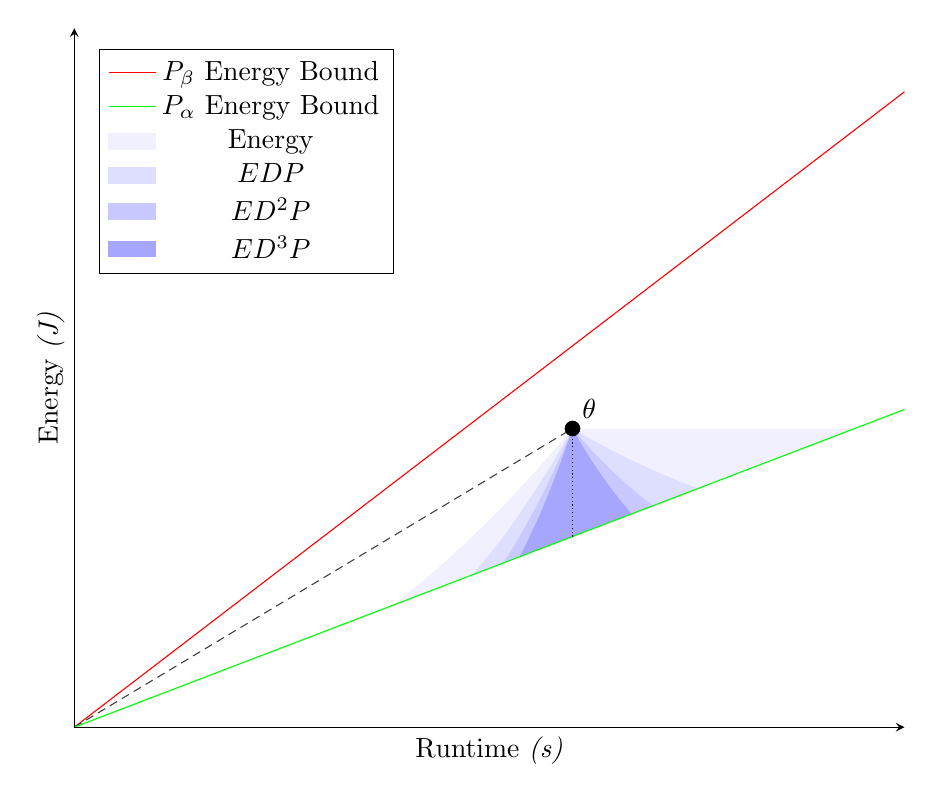
\begin{tikzpicture}
  \begin{axis}[ticks = none, 
    axis on top,
    axis x line=bottom,
    axis y line=left,
  	xlabel={Runtime \emph{(s)}},
    ylabel={Energy \emph{(J)}},    
    xmin=0, xmax=50,
    ymin=0, ymax=3300,
    width=\linewidth,
    legend style={legend pos=north west}
    ]

    %% Model Parameters %%
    \pgfmathsetmacro{\baselinepower}{30} % NOP code
    \pgfmathsetmacro{\rooflinepower}{60}
    \pgfmathsetmacro{\codepower}{47} 
    \pgfmathsetmacro{\codetime}{30}




    %% Intermezzo Values %%
    \pgfmathsetmacro{\codeenergy}{\codepower * \codetime}
    \pgfmathsetmacro{\baselineenergy}{\baselinepower * \codetime}
    \pgfmathsetmacro{\rooflineenergy}{\rooflinepower * \codetime}
    \pgfmathsetmacro{\lowdisplayline}{(2 * \baselinepower + \codepower) / 3}
    \pgfmathsetmacro{\highdisplayline}{(1 * \rooflinepower + 1 * \codepower) / 2}

    % arguments: code power, code time, x, n 
    \pgfmathdeclarefunction{metricbound}{4}{%
      \pgfmathparse{((#1 * #2^(#4 + 1)) / #3^#4)}%
    }
    \pgfmathdeclarefunction{definitionbound}{4}{%
      \pgfmathparse{((#1 / #2^(#4 + 1)) * #3^(#4 + 2))}%
    }
 
    % BETA ROOFLINE BOUND
    \addplot[color=red, domain=\pgfkeysvalueof{/pgfplots/xmin}:\pgfkeysvalueof{/pgfplots/xmax}] {\rooflinepower * x};
    \addlegendentry{$P_{\beta}$ Energy Bound}

    %const power diagonal
    \addplot[color=darkgray, densely dashed, name path=constpwr, forget plot, %forget plot prevents legend entry
            domain=\pgfkeysvalueof{/pgfplots/xmin}:\codetime] {\codepower * x}; 

    % ALPHA BASELINE BOUND 
    \addplot[color=green, name path=basebound, domain=\pgfkeysvalueof{/pgfplots/xmin}:\pgfkeysvalueof{/pgfplots/xmax}] {\baselinepower * x};
    \addlegendentry{$P_{\alpha}$ Energy Bound} 

    % Constant Time vertical dots
    %vertical
    \draw[densely dotted] ({axis cs:\codetime,\baselineenergy}) -- ({axis cs:\codetime,\codeenergy});

    % Sadly, pgfplots sucks too much to calculate cube roots
    % Domain values are calculated with a ruby script in tools

    %% Energy Area %%
    \addplot[name path=energy, draw=none, domain=19.14894:47, forget plot]{ min(definitionbound(\codepower, \codetime, x, 0),metricbound(\codepower, \codetime, x, 0))};
    \addplot[blue!6] fill between[of=energy and basebound];
    \addlegendentry{Energy}

    %% Energy Delay Product Area %% 
    \addplot[name path=edp, draw=none, domain=23.96806:37.54997, forget plot] { min(definitionbound(\codepower, \codetime, x, 1),metricbound(\codepower, \codetime, x, 1))};
    \addplot[blue!13] fill between[of=edp and basebound];
    \addlegendentry{$EDP$}

    %% Energy Delay Squared Product Area ##
    \addplot[name path=edtwop, draw=none, domain=25.83028:34.84283, forget plot] { min(definitionbound(\codepower, \codetime, x, 2),metricbound(\codepower, \codetime, x, 2))};
    \addplot[blue!21] fill between[of=edtwop and basebound];
    \addlegendentry{$ED^2P$}

    %% Energy Delay Cubed Product Area ##
    \addplot[name path=edthreep, draw=none, domain=26.81496:33.56336, forget plot] { min(definitionbound(\codepower, \codetime, x, 3),metricbound(\codepower, \codetime, x, 3))};
    \addplot[blue!35] fill between[of=edthreep and basebound];
    \addlegendentry{$ED^3P$}




     \node[circle,fill,inner sep=2pt] at (axis cs:\codetime,\codeenergy) {};
    \node[above right] at (axis cs:\codetime,\codeenergy) {$\theta$};
  \end{axis}
\end{tikzpicture}

\caption{Multiple Metric Code Optimization Spaces}
\label{fig:multimetric-technique}
\end{figure}
